\documentclass[xcolor=dvipsnames]{beamer}
\usepackage[polish]{babel}
\usepackage[utf8]{inputenc}
\usepackage[OT4]{fontenc}
\usepackage{graphics}
\usepackage{subfigure}

\usetheme{Berlin}
%\usecolortheme[RGB={154,63,31}]{structure}
\useinnertheme{rounded}
\useoutertheme{infolines}
\setbeamertemplate{blocks}[rounded][shadow=true]

\newenvironment{ramka}{\begin{frame}}
{
		\end{frame}
}

\begin{document}
	\title[Embedded Linux]{Konstrukcja platformy sprzętowej dla potrzeb wbudowanego systemu Linux}
	\author[Jakub Odias]{Autor: Jakub Odias\\\vspace{5pt}Promotor: dr inż. Krzysztof Tokarz}
	
	\begin{frame}
		\begin{figure}[b]
			
\includegraphics[scale=0.15]{text/img/polsl.png} 
		\end{figure}
		\vspace{-20pt}
		\center{Praca dyplomowa magisterska}
		\vspace{10pt}
		\titlepage
		
	\end{frame}
	
	\section{Wstęp}
	%\subsection{Agenda}
	%\begin{ramka}
	%	\frametitle{Agenda}
	%	\tableofcontents
	%\end{ramka} 
	
	\subsection{Embedded Linux}
	\begin{ramka}
		\frametitle{Embedded Linux}
		\begin{block}{Co to jest wbudowany Linux?}
			\begin{itemize}
				\item<2-> System przystosowany specjalnie dla potrzeb urządzeń posiadających ograniczone zasoby
				\item<3-> Jądro jest znacznie okrojone w stosunku do tych używanych na serwerach czy desktopach
				\item<4-> Posiada aplikacje zoptymalizowane do konkretnych celów
			\end{itemize}
		\end{block}
	\end{ramka} 
	
	\subsection{Temat projektu}
	\begin{ramka}
		\frametitle{Temat projektu}
		\begin{block}{Platforma sprzętowa dla potrzeb wbudowanego systemu Linux}
			\begin{itemize}
			\item<2->Celem projektu jest stworzenie platformy sprzętowej umożliwiającej podłączenie sieci Ethernet, wyświetlacza graficznego LCD, urządzeń USB oraz kart pamięci SD/MMC.\\
			\item<3->Płytka będzie docelowo wykorzystana jako multimedialne urządzenie umożliwiające odtwarzanie utworów muzycznych. Interfejs użytkownika będzie dostępny za pomocą sieci Ethernet lub np. dołączanej klawiatury USB.
			\end{itemize}
		\end{block}
	\end{ramka} 
	
	\section{Hardware}
	%\subsection{Mikrokontroler}
	%\begin{ramka}
	%	\frametitle{Hardware}
	%	\begin{block}{Mikrokontroler z rodziny ARM - Atmel AT91RM9200}
	%		\begin{itemize}
	%			\item<2-> 200MIPS @ 180MHz, Memory Management Unit
	%			\item<3-> EBI - wsparcie dla pamięci SDRAM, Compact Flash, NAND flash
	%			\item<4-> Ethernet 10/100 Mbps
	%			\item<5-> Działa jako host i urządzenie USB
	%			\item<6-> Interfejs dla kart SD/MMC
	%			\item<7-> SPI, 4*USART, TWI, RTC
	%		\end{itemize}
	%	\end{block}
	%\end{ramka} 
	
	\subsection{Zastosowane układy}
	\begin{ramka}
		\frametitle{Hardware}
		\begin{itemize}
			\item<1-> Mikrokontroler ARM9 AT91RM9200 - 210MHz
			\item<1-> 64MB SDRAM
			\item<1-> 256kB pamięci Serial Dataflash (bootloader)
			\item<1-> 2 złącza kart pamięci SD/MMC
			\item<1-> Ethernet 10/100 Mbps
			\item<1-> Kontroler LCD SSD1906 + wyświetlacz z Sony PSP
			\item<1-> Przetwornik audio
			\item<1-> Host USB
			\item<1-> JTAG, UART
		\end{itemize}
	\end{ramka} 
	
	\subsection{Projekt platformy}
	\begin{ramka}
		\frametitle{Schemat elektryczny}
		\begin{figure}[h]
			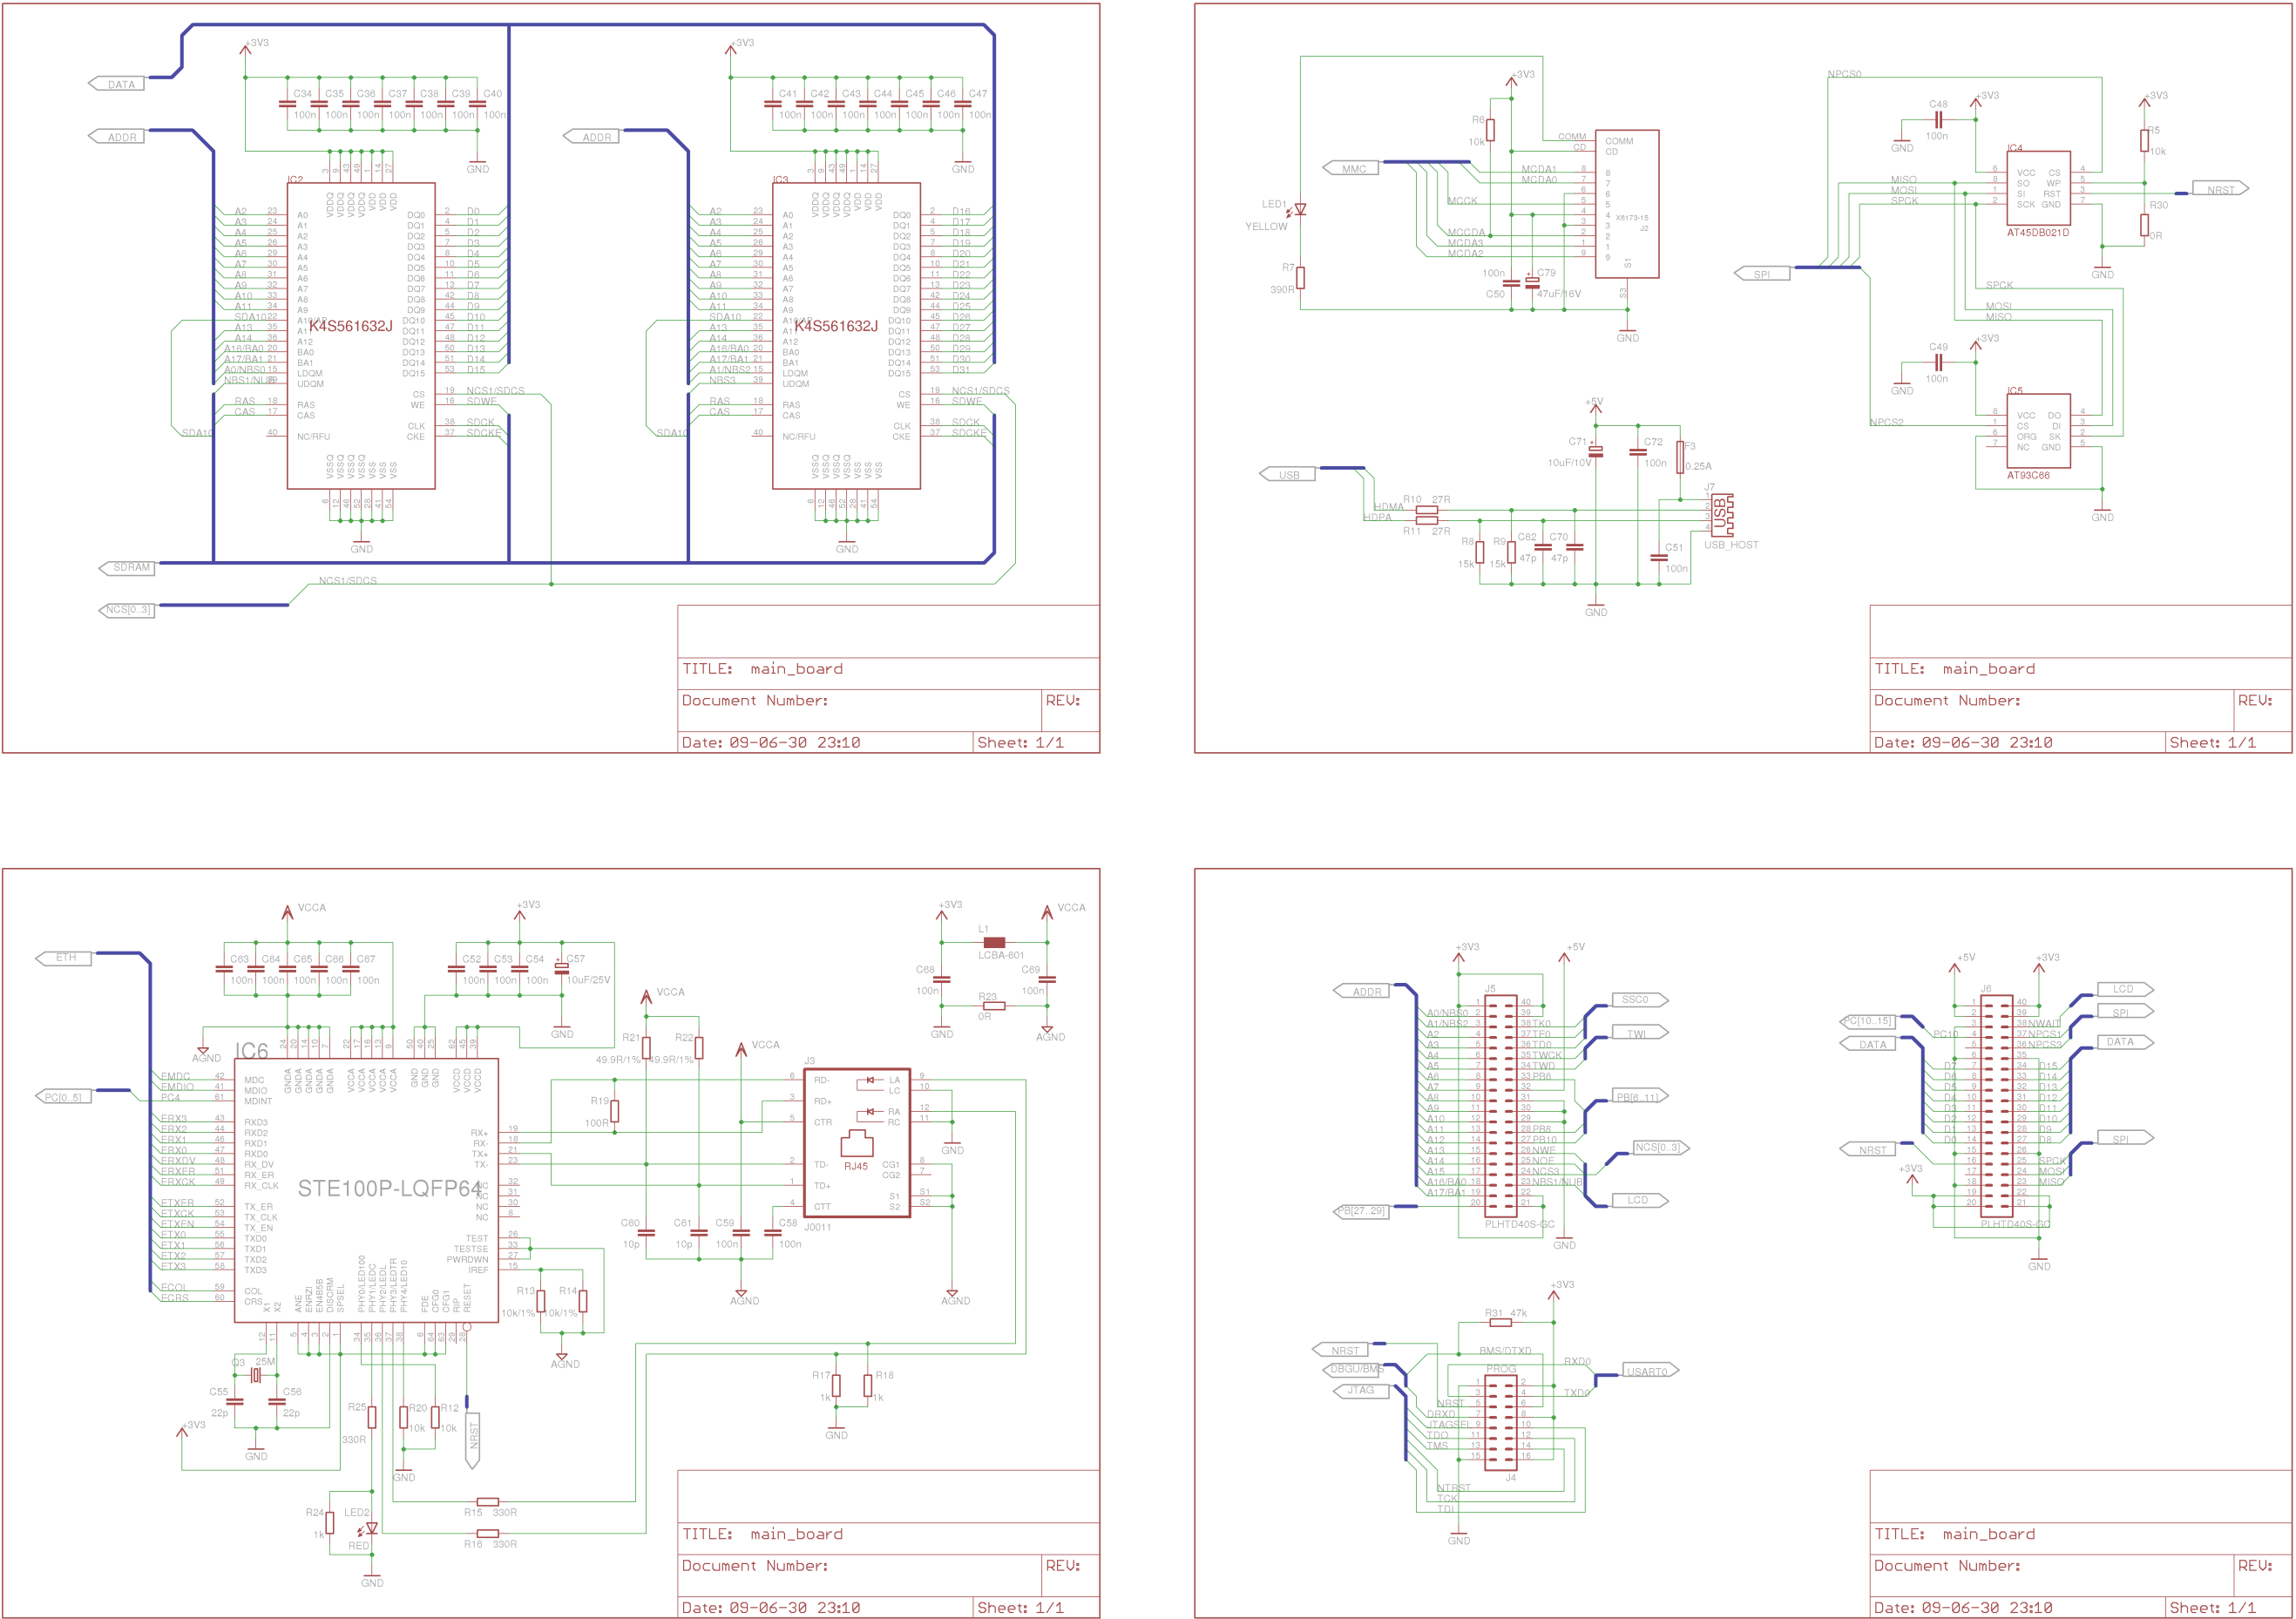
\includegraphics[scale=0.4]{text/img/main_sch.png} 
		\end{figure}
	\end{ramka}
	
	\begin{ramka}
		\frametitle{Projekt PCB}
		\begin{figure}[h]
			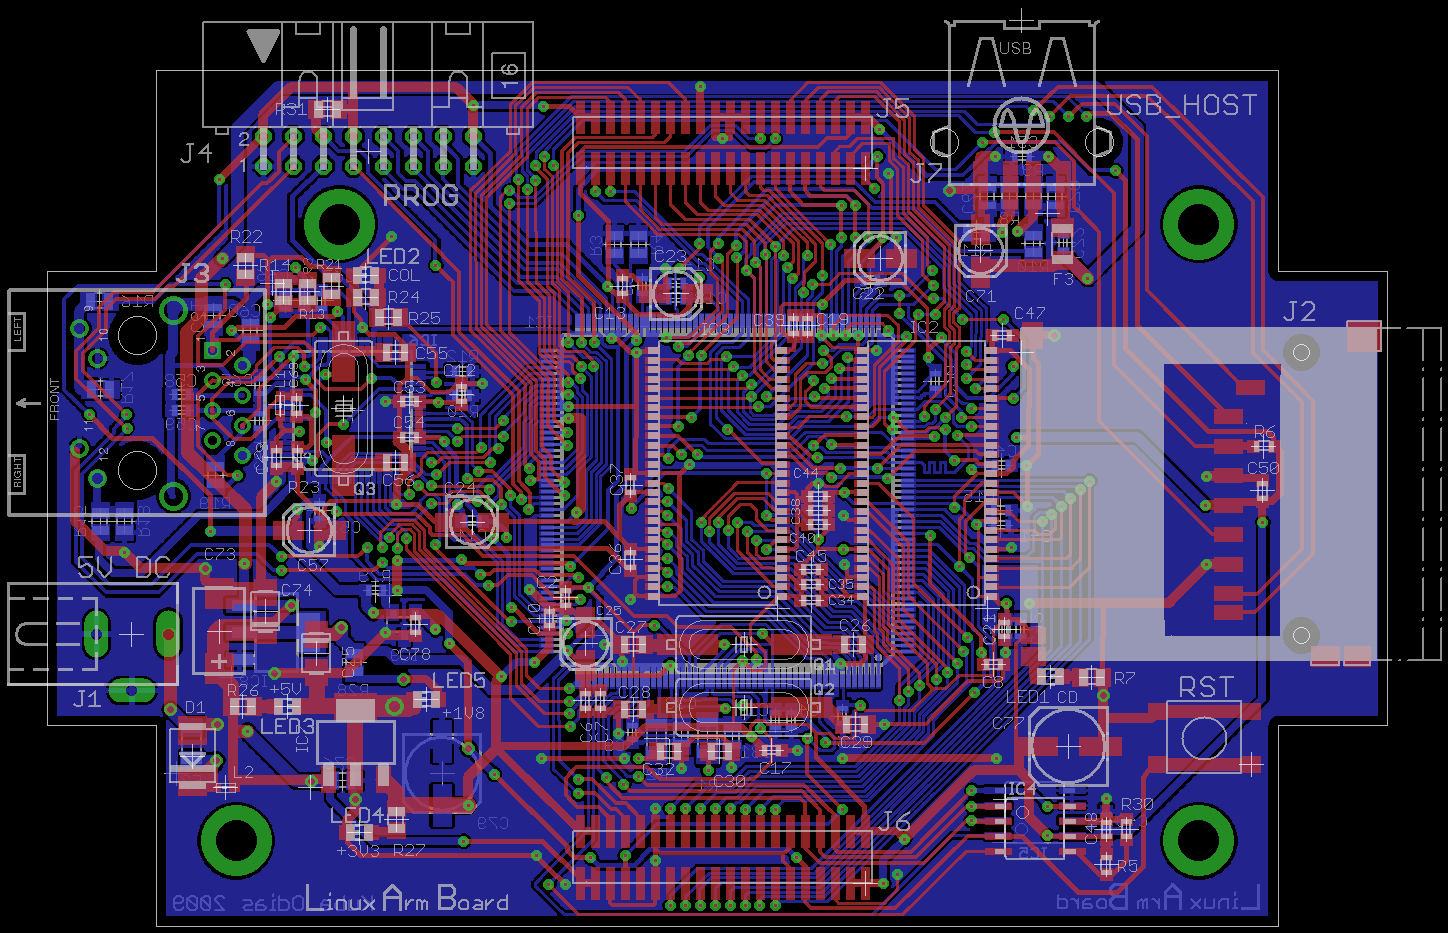
\includegraphics[scale=0.7]{text/img/main_brd.png} 
		\end{figure}
	\end{ramka}
	
	\begin{ramka}
		\frametitle{Gotowy układ}
		\begin{figure}[h]
			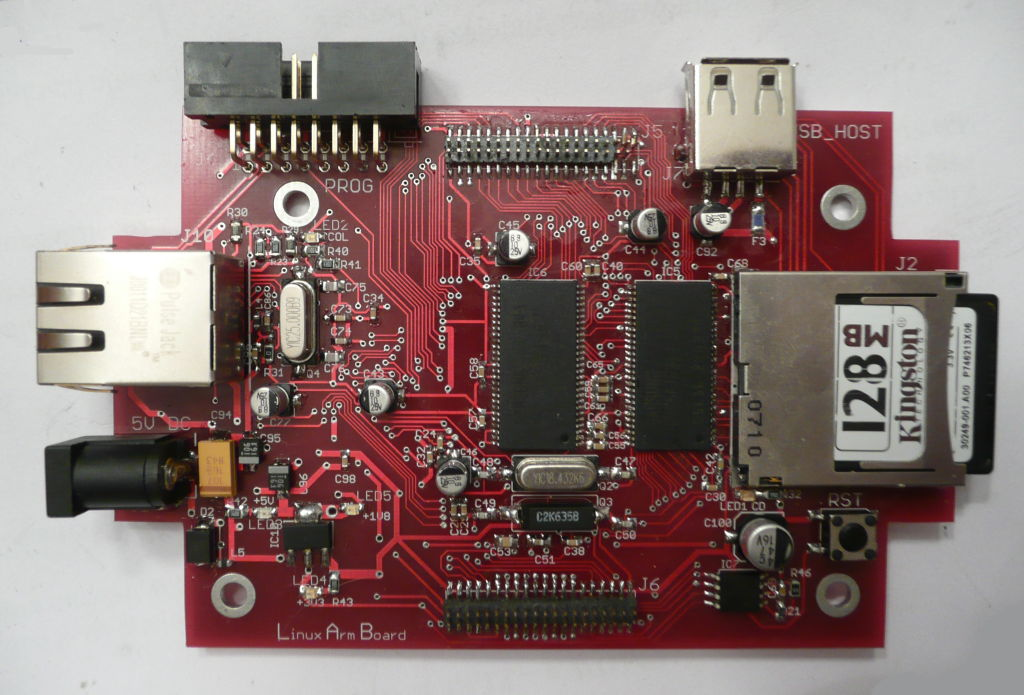
\includegraphics[scale=0.5]{text/img/pcb1_ready_top.jpg} 
		\end{figure}
	\end{ramka}
	
		\begin{ramka}
		\frametitle{Gotowy układ}
		\begin{figure}[h]
			\subfigure{\includegraphics[scale=0.23]{text/img/pcb2_ready_top.jpg}}
			\hspace{10pt}
			\subfigure{\includegraphics[scale=0.23]{text/img/pcb2_ready_bottom.jpg}}\\
			%\vspace{10pt}
			\subfigure{\includegraphics[scale=0.23]{text/img/pcb1_ready_bottom.jpg}}
			\hspace{10pt}
			\subfigure{\includegraphics[scale=0.23]{text/img/project.jpg}}
		\end{figure}
	\end{ramka}
	
	\section{Software}
	\subsection{Bootloader}
	\begin{ramka}
		\frametitle{Software}
		\begin{block}{Proces uruchamiania}
			\begin{itemize}
				\item<2-> bootloader inicjalizujący - inicjalizacja pamięci i układów peryferyjnych oraz podstawowe testy
				\item<3-> bootloader główny (U-boot) - inicjalizacja sieci i/lub karty pamięci SD/MMC oraz wczytanie kernela
				\item<4-> jądro Linuksa
			\end{itemize}
		\end{block}
	\end{ramka}
	
	\subsection{Dystrybucja}
	\begin{ramka}
		\frametitle{Software}
		\begin{block}{Dystrybucja}
			\begin{itemize}
				\item<1-> $\mu$cLinux
				\item<1-> RTLinux
				\item<1-> standardowe dystrybucje np. Debian
			\end{itemize}
		\end{block}
	\end{ramka}
	
	\subsection{Sterowniki urządzeń}
	\begin{ramka}
		\frametitle{Software}
		\begin{block}{Sterowniki urządzeń}
			\begin{itemize}
				\item<1-> kontroler LCD
				\item<1-> moduł Bluetooth
				\item<1-> przetwornik audio
			\end{itemize}
		\end{block}
	\end{ramka}
	
	\section*{Podsumowanie}
	\begin{ramka}
		\begin{center}
			\textbf{\Large{Dziękuję za uwagę}}
		\end{center}
	\end{ramka}

\end{document}